%%%
 % File:     buffer_overflow.tex
 % Author:   Hackademics Forum <hackademicsforum6@gmail.com>
 % Project:  MindMap des vulnérabilités
 % Released: 03/08/2016
%%%

%!TeX root = main.tex
%!TeX encoding = UTF-8
%!TeX program = pdflatex
%!TeX spellcheck = fr_FR

%%%
 % Vulnérabilités Buffer Overflow
%%%
\newpage
\section{Dépassement de tampon (Buffer Overflow)}\label{vulnerabilites:applicatives:buffer-overflow}

Un Buffer Overflow ou dépassement de tampon se produit lorsque un programme ou un processus tente de stocker plus de données dans une mémoire tampon (stockage temporaire) )que prévue par celle-ci. Ces mémoires tampon sont prévues pour accueillir une quantité limitée de données. les informations supplémentaires qui doivent bien être stockées quelque part se retrouvent dans des tampons adjacents. Les données déjà stockées dans ces tampons sont à ce moment écrasées et endommagée. Bien que cela puisse également se produire accidentellement en raison d'une erreur de programmation les dépassements de tampon sont de plus en plus utilisés pour volontairement corrompre les données. Dans des attaques ciblées par débordement de tampon, ces informations complémentaires peuvent contenir du code malveillant qui déclenchera des actions spécifiques sur le système attaqué. Par exemple le code peut contenir des instructions qui peuvent endommager des fichiers sur le pc, simplement modifier des données ou mener au vol de certains renseignements intéressants.


\subsection{Stack Overflow}\label{vulnerabilites:applicatives:buffer-overflow:stack}

Chez les processeurs X86, le STACK commence a l’extrémité supérieure de la mémoire (ex:0xffffffff) et pousse vers le bas (vers 0x00000000). Le mot STACK viens de l'anglais et veut dire PILE. Il se nomme ainsi car il se comporte en LIFO (Last In First Out): si quelque chose est ajouté (PUSH,écriture), la PILE est augmentée, au contraire si quelque chose est lu (POP), la PILE est abaissée: l'élément est lu et supprimé. Il existe une troisième méthode nommée TOP ou PEEK, ou l'élément est simplement lu mais pas supprimé. Le pointeur de PILE (ESP) est toujours à la dernière adresse de la PILE.

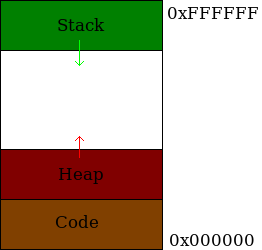
\includegraphics[scale=0.3]{Application/assets/stack.png}

\subsection{Heap Overflow}\label{vulnerabilites:applicatives:buffer-overflow:heap}

...

\endinput
